\documentclass[12pt,a4paper,titlepage]{article}

\usepackage{preamble}

\title{Représentation  Temps-Fréquence : travaux pratiques}
\author{Yassine Jamoud, Samy Haffoudhi}
\date{\today}

\begin{document}

\maketitle

\setcounter{section}{1}

\section{Représentation temps-fréquence de signaux simulés}

\subsection{Génération de signaux}

Représentons l'allure temporelle, la phase instantanée et la fréquence instantanée des signaux
mono-composantes $x_1$ et $x_2$ :

\begin{figure}[H]
    \caption{allure temporelle, phase et fréquence instantanée de $x_1$ et $x_2$}
    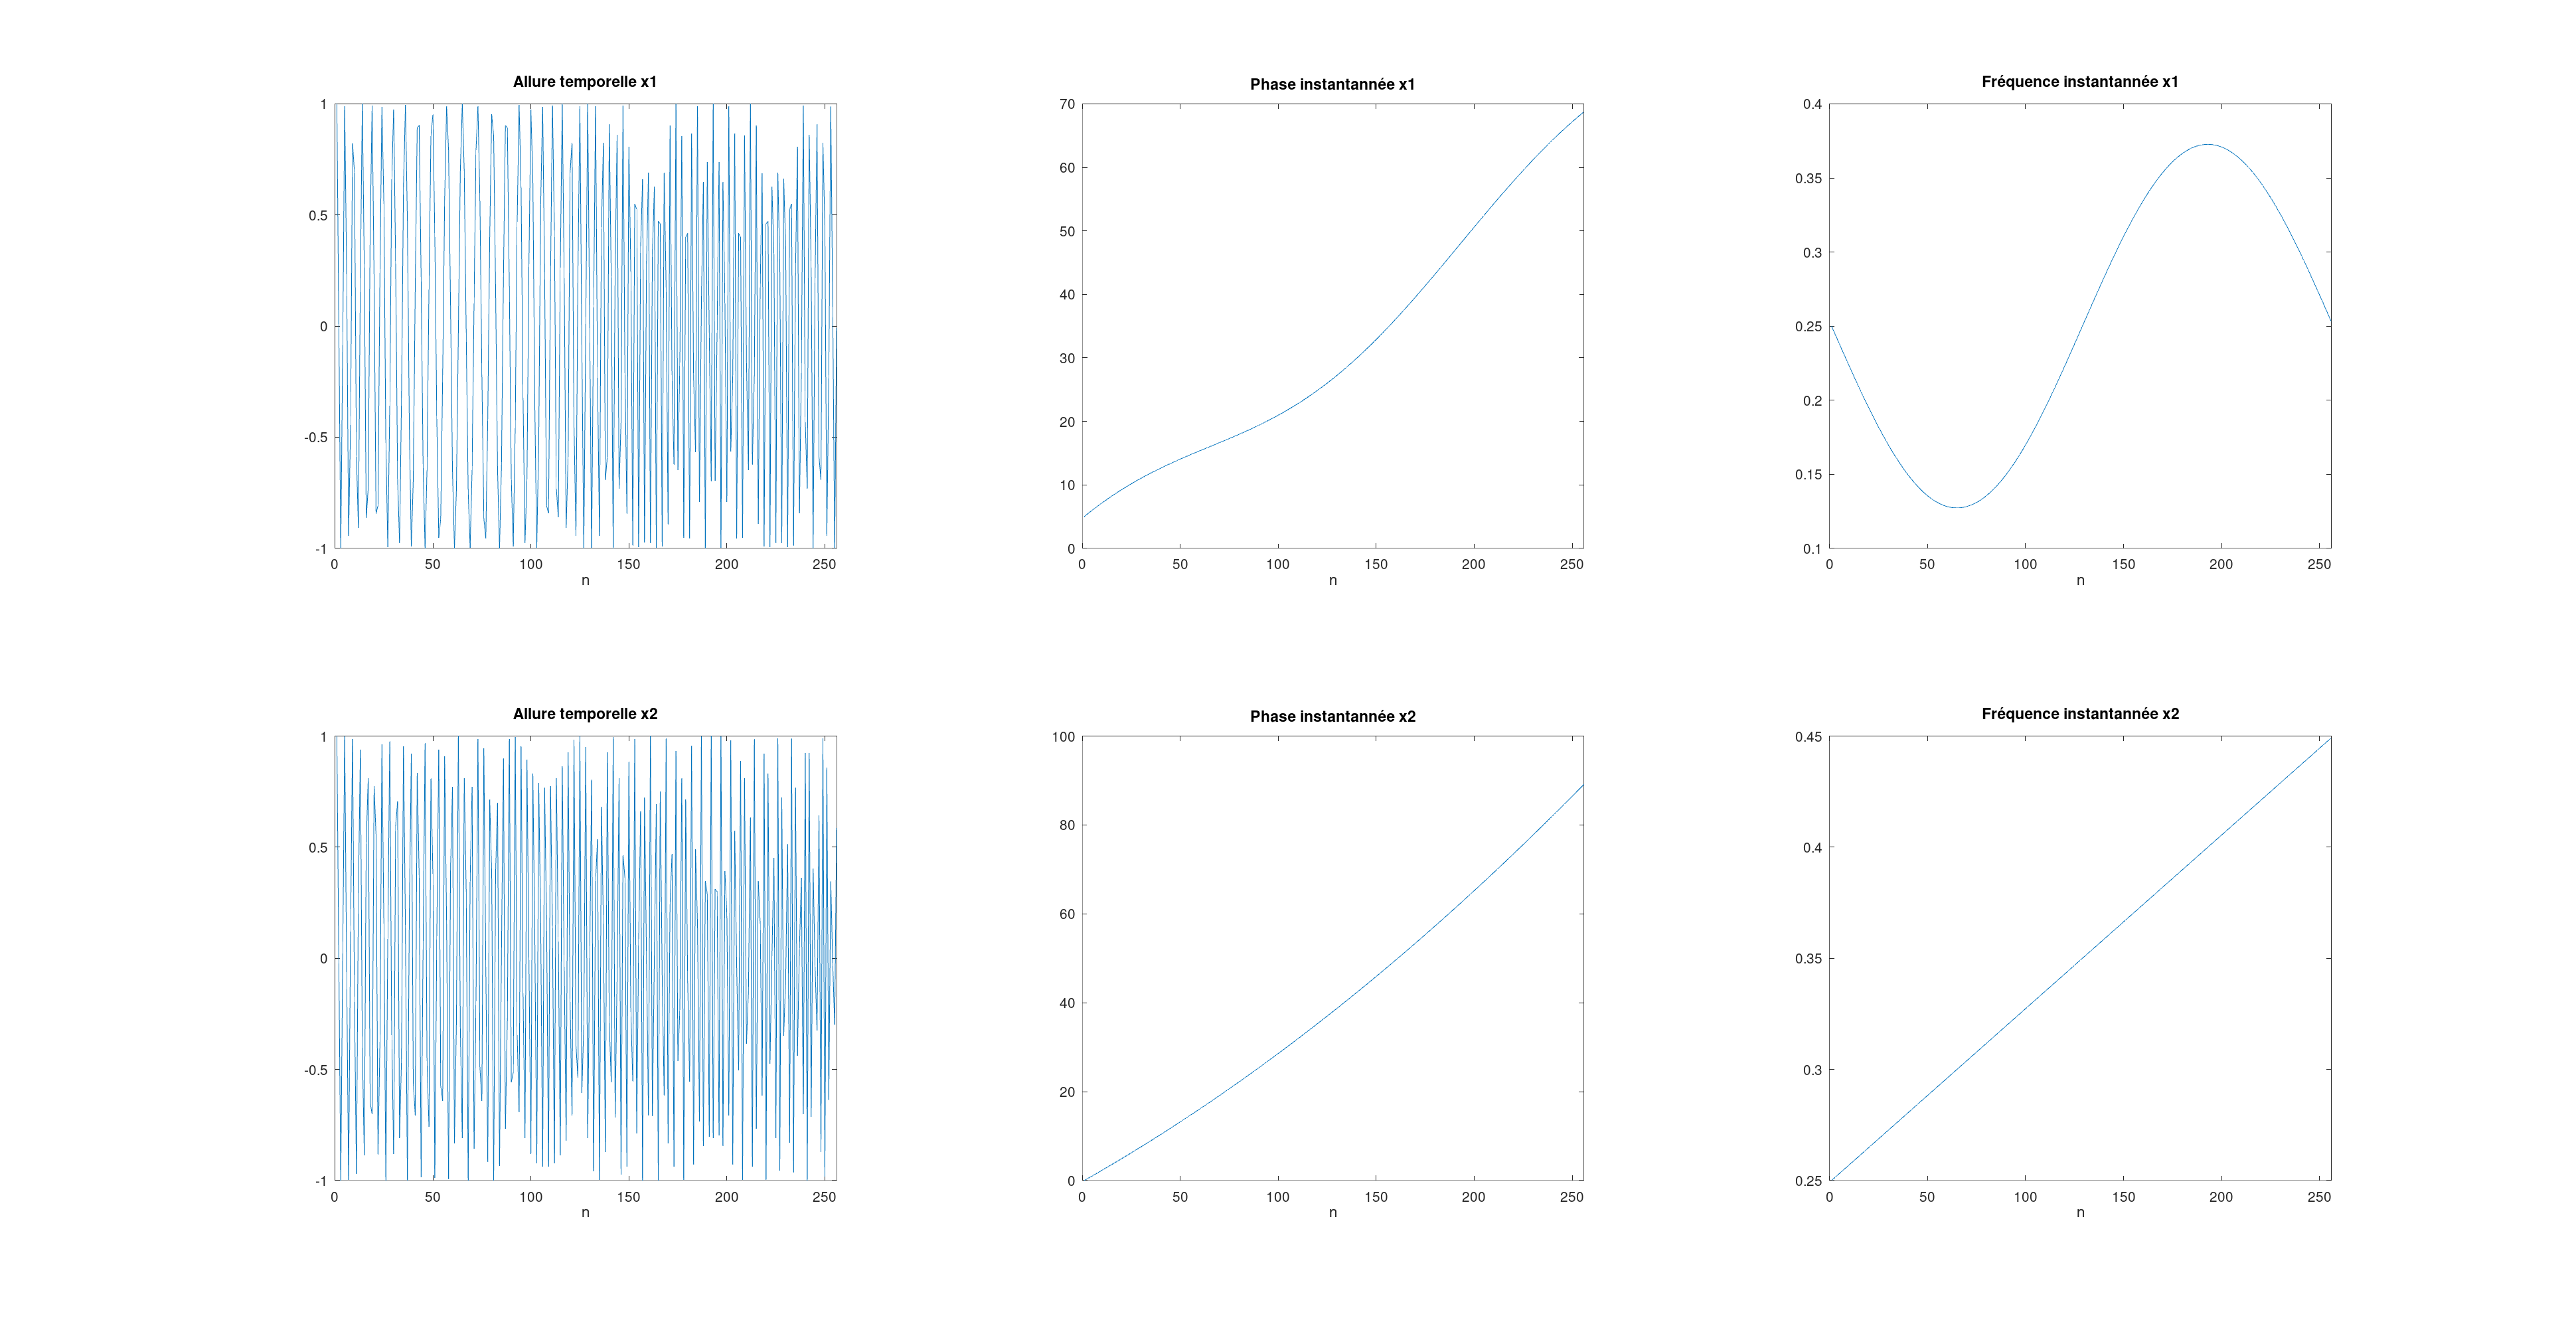
\includegraphics[width=\textwidth]{ex1q1}
    \centering
\end{figure}

Représentons maintenant l'allure du signal $x_3$, somme de quatre atomes gaussiens :

\begin{figure}[H]
    \caption{Allure temporelle du signal $x_3$}
    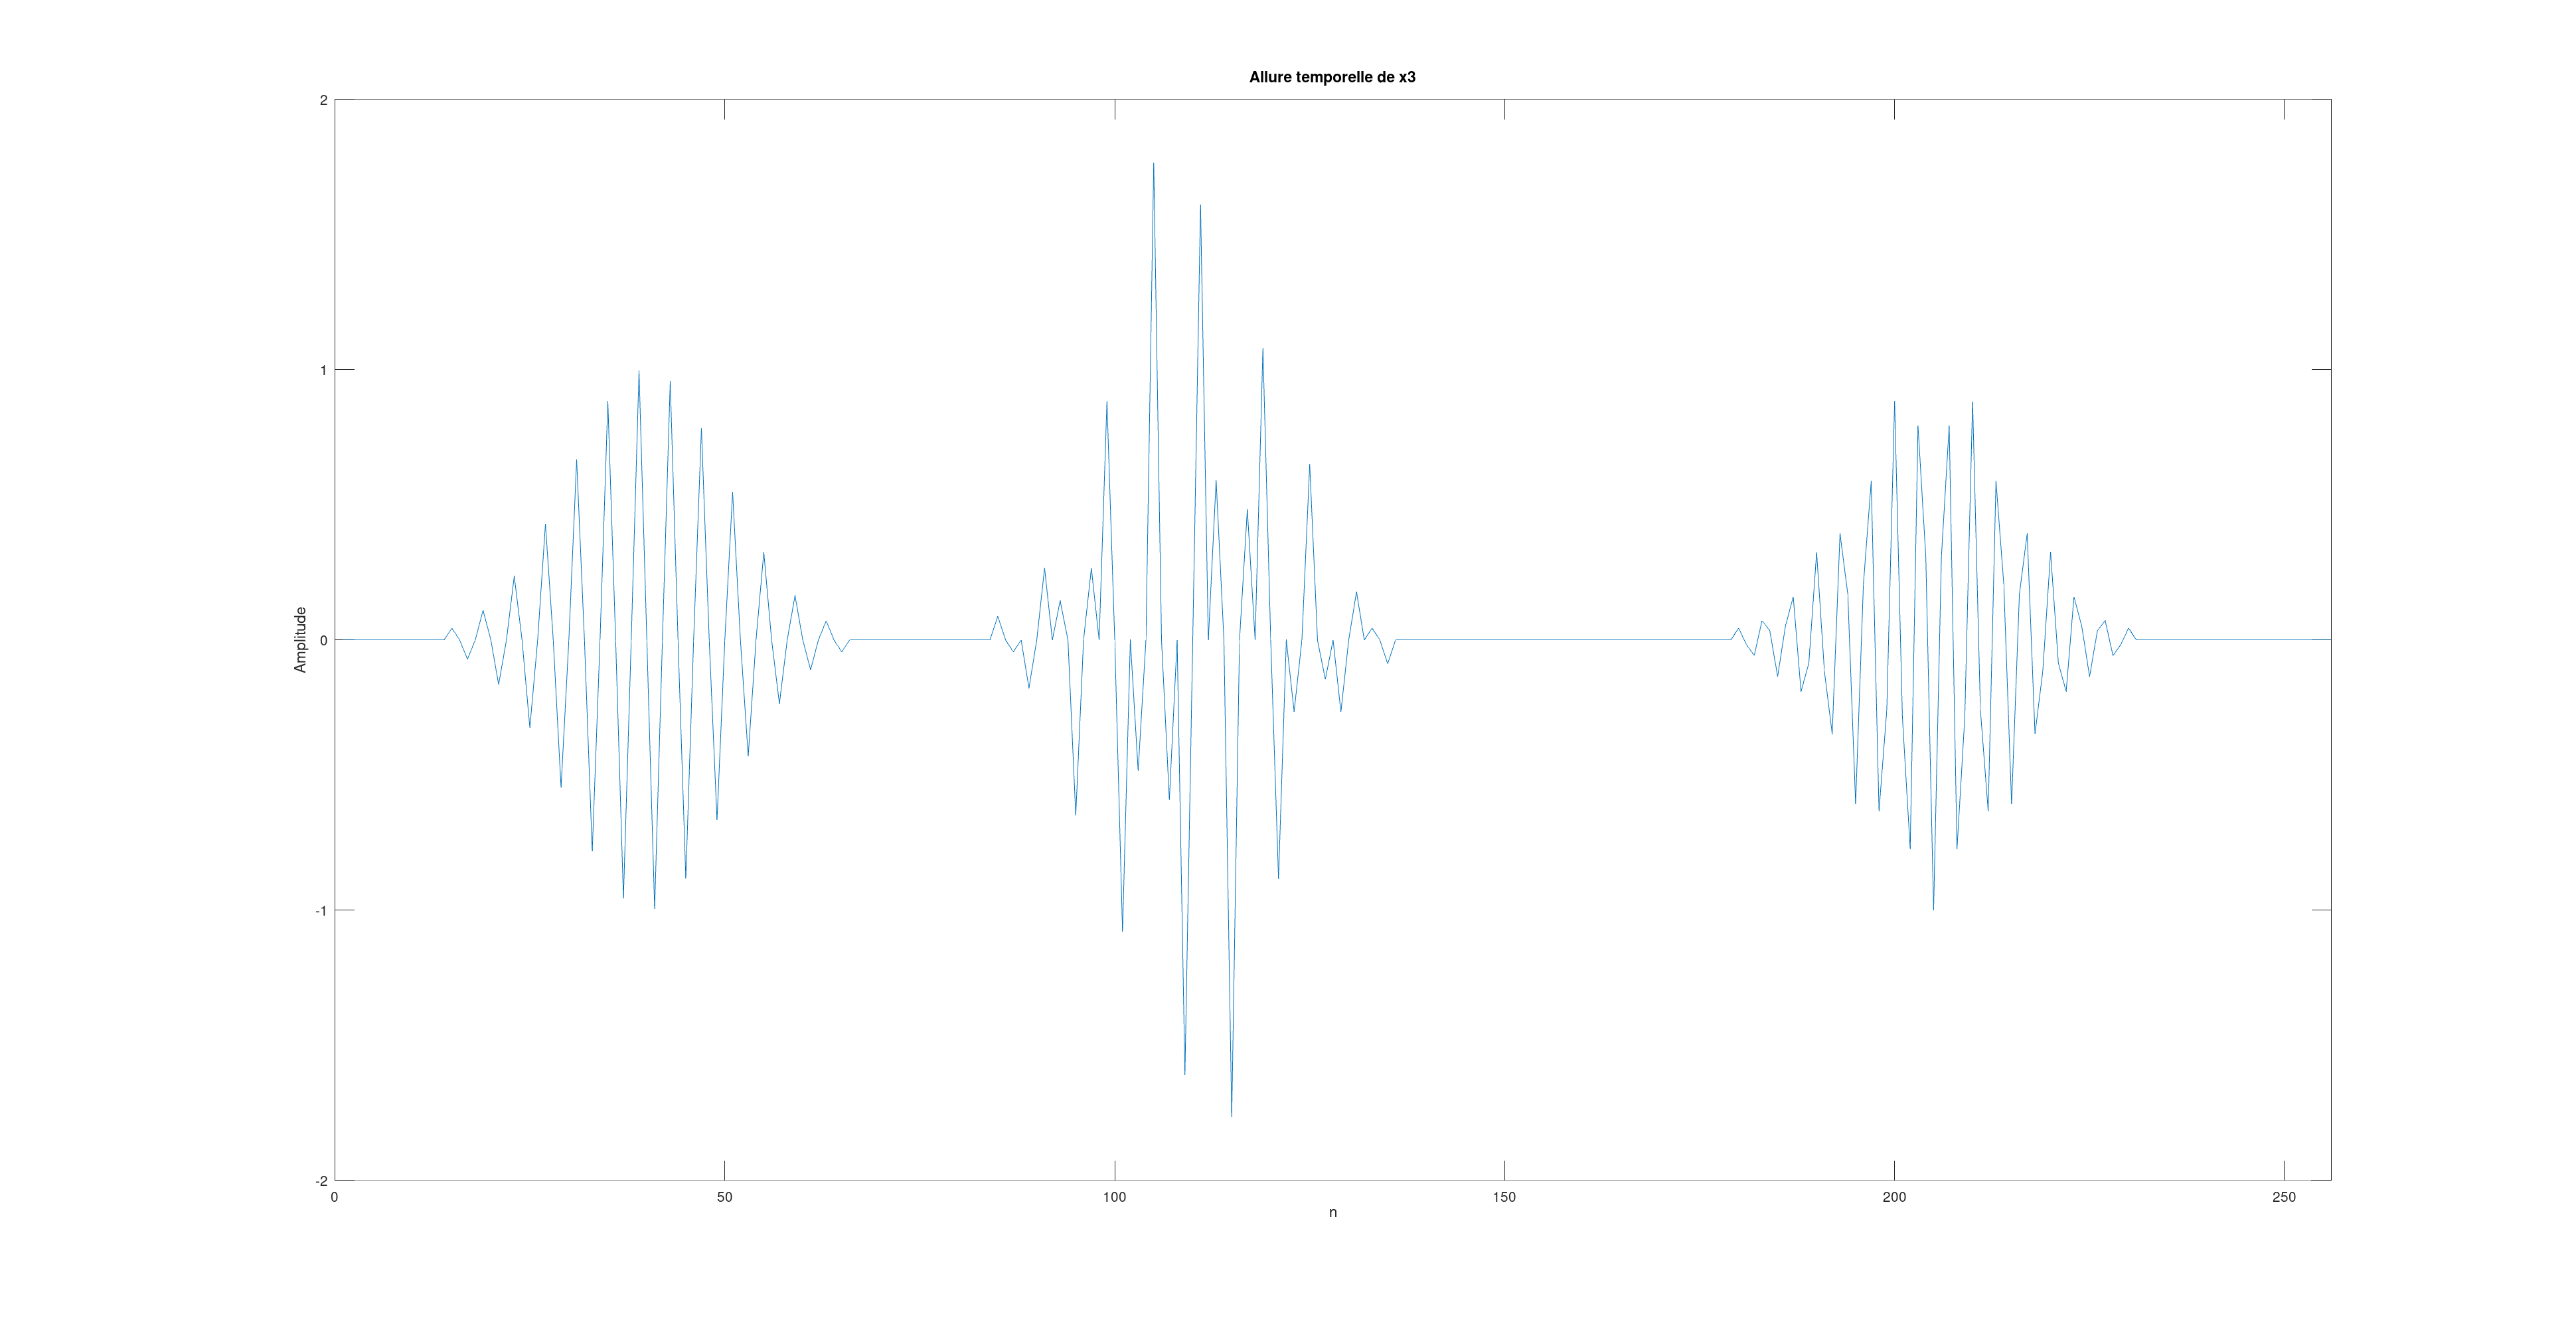
\includegraphics[width=\textwidth]{ex1q2}
    \centering
\end{figure}

Nous avons obtenus ces différentes figures à l'aide du script présenté en \textbf{Annexe A} et par le calcul
au préalable de $f_i(t) = \frac{d\phi_i(t)}{dt}$.

\subsection{Représentation temps-fréqyence}

Pour chaque signal nous allons maintenant représenter :

\begin{itemize}
    \item{Le spectrogramme en utilisant une fenêtre de Hamming de longueur \texttt{Nh} = 17, 33, 65
        et 129.}
    \item{La transformée de Wigner-Ville}
    \item{La transformée de pseudo-Wigner-Ville en utilisant uen fenêtre de Kaiser avec \texttt{Nh}
        = 63.}
    \item{La transformée de pseudo-Wigner-Ville lissée avec des fenêtres de Kaiser de longueur
        \texttt{Ng} = 33 et \texttt{Nh} = 63, puis \texttt{Ng} = 15 et \texttt{Nh} = 63.}
\end{itemize}

On obtient les figures suivantes :

\begin{appendices}

    \section{Scripts Représentation temps-fréquence de signaux simulés}

    \lstinputlisting[language=Matlab]{../ex1.m}

\end{appendices}

\end{document}
